\documentclass{standalone}
\usepackage{tikz}
\usetikzlibrary{patterns, positioning}
\usepackage[sfdefault]{ClearSans} %% option 'sfdefault' activates Clear Sans as the default text font
\usepackage[T1]{fontenc}

\begin{document}
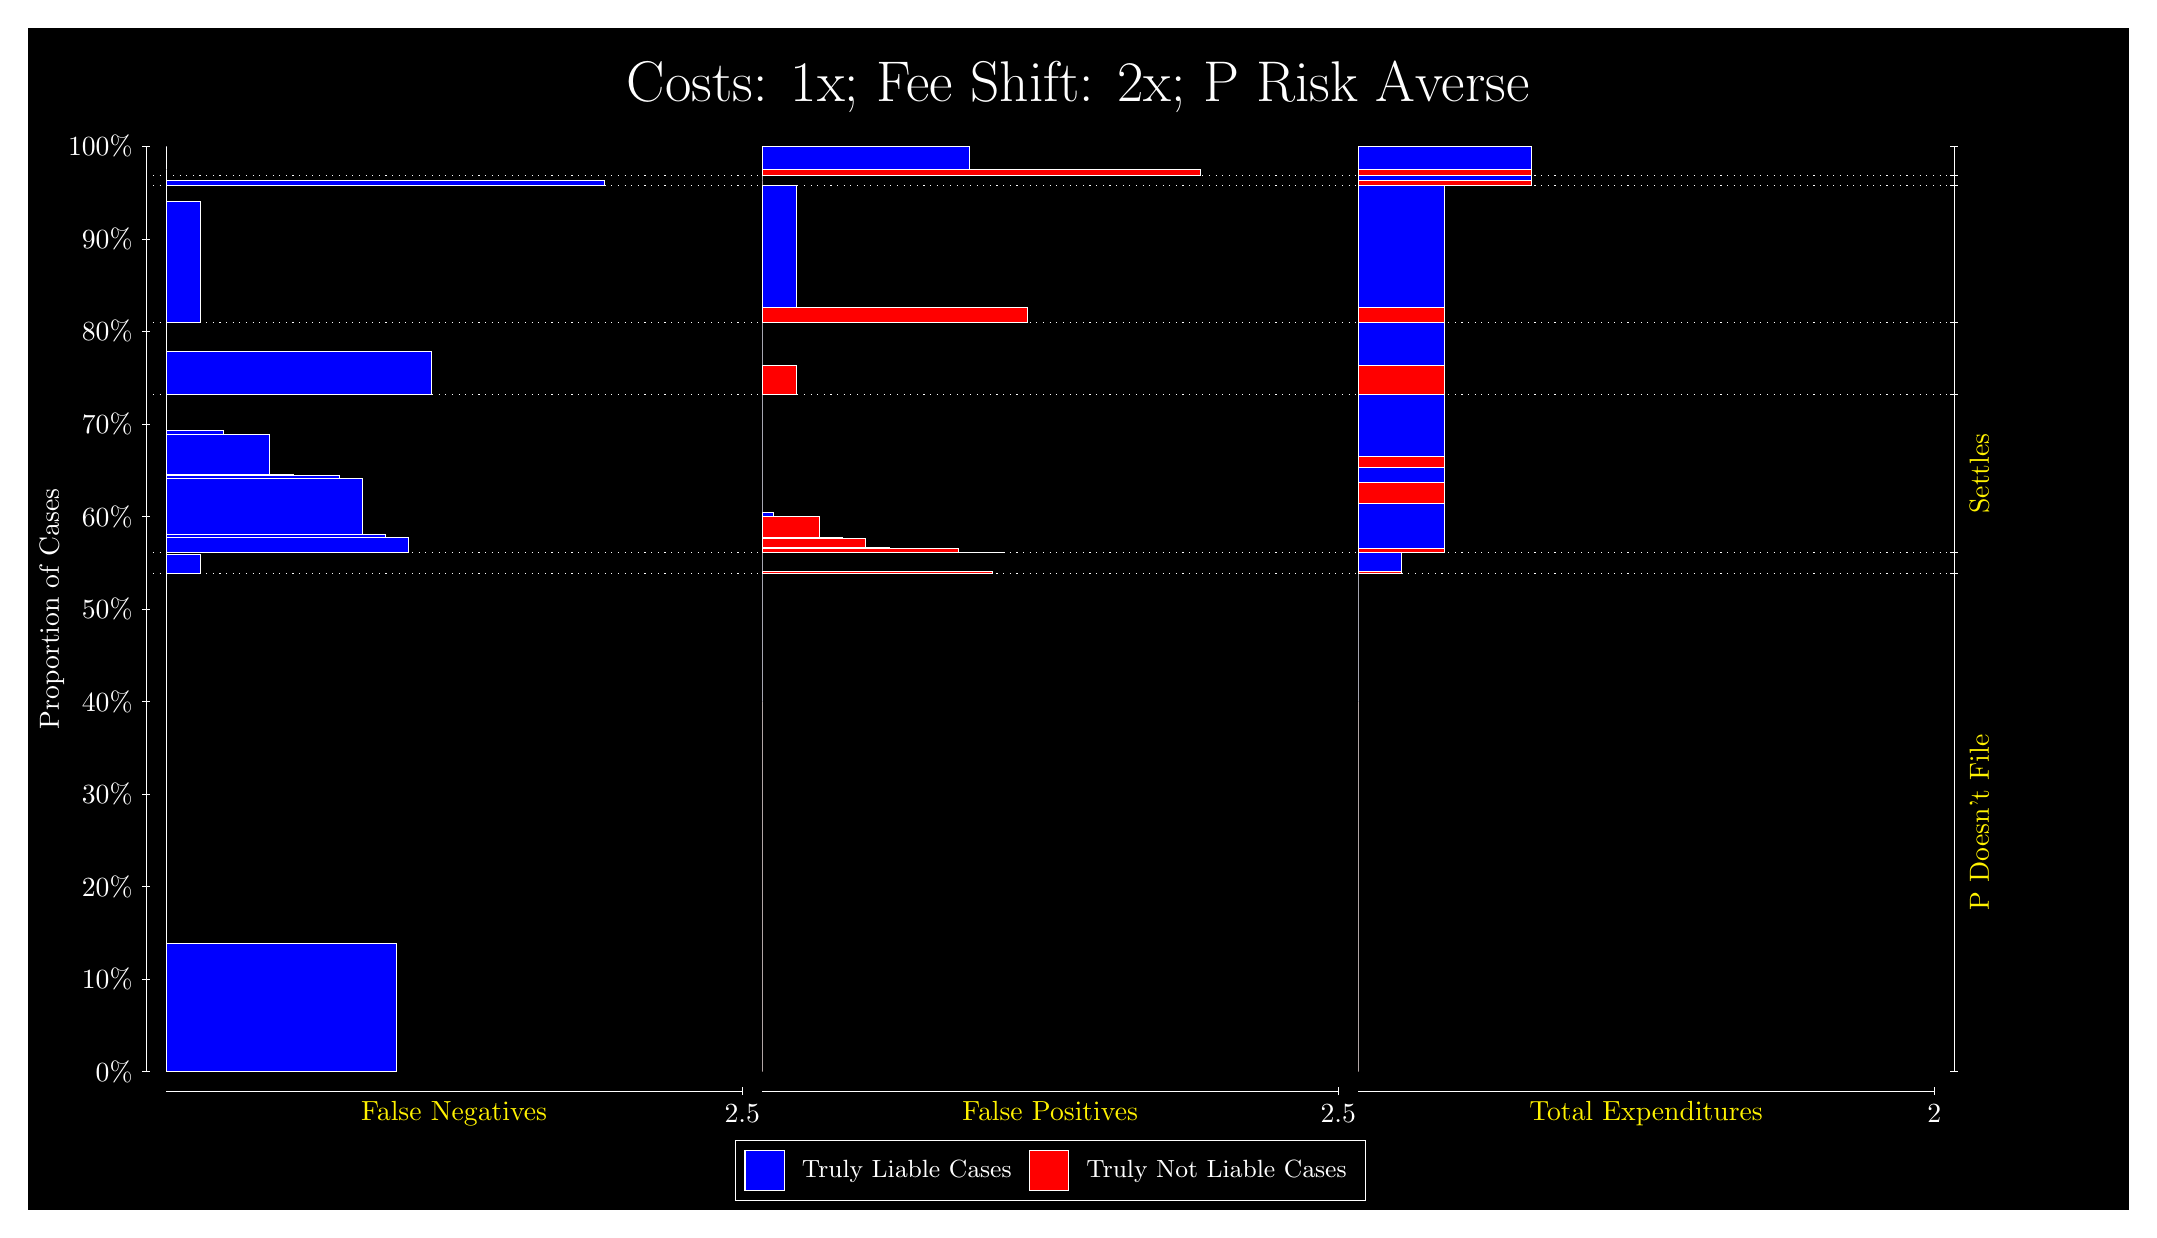
\begin{tikzpicture}
\draw[fill=black] (0,0) rectangle (26.667,15);
\draw[text=white] (0,13.5) rectangle (26.667,15) node[midway] {\huge Costs: 1x; Fee Shift: 2x; P Risk Averse};
\draw[white, very thin] (1.5,1.75) -- (1.5,13.5);
\node[rotate=90, text=white, anchor=center] at (0.3, 7.625) {Proportion of Cases};
\draw[white, very thin] (1.45,1.75) -- (1.55,1.75);
\node[text=white, anchor=east] at (1.45, 1.75) {0\%};
\draw[white, very thin] (1.45,2.925) -- (1.55,2.925);
\node[text=white, anchor=east] at (1.45, 2.925) {10\%};
\draw[white, very thin] (1.45,4.1) -- (1.55,4.1);
\node[text=white, anchor=east] at (1.45, 4.1) {20\%};
\draw[white, very thin] (1.45,5.275) -- (1.55,5.275);
\node[text=white, anchor=east] at (1.45, 5.275) {30\%};
\draw[white, very thin] (1.45,6.45) -- (1.55,6.45);
\node[text=white, anchor=east] at (1.45, 6.45) {40\%};
\draw[white, very thin] (1.45,7.625) -- (1.55,7.625);
\node[text=white, anchor=east] at (1.45, 7.625) {50\%};
\draw[white, very thin] (1.45,8.8) -- (1.55,8.8);
\node[text=white, anchor=east] at (1.45, 8.8) {60\%};
\draw[white, very thin] (1.45,9.975) -- (1.55,9.975);
\node[text=white, anchor=east] at (1.45, 9.975) {70\%};
\draw[white, very thin] (1.45,11.15) -- (1.55,11.15);
\node[text=white, anchor=east] at (1.45, 11.15) {80\%};
\draw[white, very thin] (1.45,12.325) -- (1.55,12.325);
\node[text=white, anchor=east] at (1.45, 12.325) {90\%};
\draw[white, very thin] (1.45,13.5) -- (1.55,13.5);
\node[text=white, anchor=east] at (1.45, 13.5) {100\%};

\draw[white, very thin] (24.457,1.75) -- (24.457,13.5);
\draw[white, very thin] (24.407,1.75) -- (24.507,1.75);
\node[anchor=west] at (24.407, 1.75) {};
\draw[white, very thin] (24.407,8.0771) -- (24.507,8.0771);
\node[anchor=west] at (24.407, 8.0771) {};
\draw[white, very thin] (24.407,8.3422) -- (24.507,8.3422);
\node[anchor=west] at (24.407, 8.3422) {};
\draw[white, very thin] (24.407,10.349) -- (24.507,10.349);
\node[anchor=west] at (24.407, 10.349) {};
\draw[white, very thin] (24.407,11.26) -- (24.507,11.26);
\node[anchor=west] at (24.407, 11.26) {};
\draw[white, very thin] (24.407,13.002) -- (24.507,13.002);
\node[anchor=west] at (24.407, 13.002) {};
\draw[white, very thin] (24.407,13.135) -- (24.507,13.135);
\node[anchor=west] at (24.407, 13.135) {};
\draw[white, very thin] (24.407,13.5) -- (24.507,13.5);
\node[anchor=west] at (24.407, 13.5) {};

\draw[white, very thin, fill=blue] (1.75,1.75) rectangle (4.6775,3.3784);
\draw[white, very thin, fill=red] (1.75,3.3784) rectangle (1.75,8.0771);
\draw[white, very thin, fill=blue] (1.75,8.0771) rectangle (2.1891,8.3179);
\draw[white, very thin, fill=red] (1.75,8.3179) rectangle (1.75,8.3422);
\draw[white, very thin, fill=blue] (1.75,8.3422) rectangle (4.8239,8.5328);
\draw[white, very thin, fill=blue] (1.75,8.5328) rectangle (4.5312,8.5682);
\draw[white, very thin, fill=blue] (1.75,8.5682) rectangle (4.2384,9.2817);
\draw[white, very thin, fill=blue] (1.75,9.2817) rectangle (3.9457,9.3231);
\draw[white, very thin, fill=blue] (1.75,9.3231) rectangle (3.6529,9.3273);
\draw[white, very thin, fill=blue] (1.75,9.3273) rectangle (3.3602,9.3295);
\draw[white, very thin, fill=blue] (1.75,9.3295) rectangle (3.0674,9.8444);
\draw[white, very thin, fill=blue] (1.75,9.8444) rectangle (2.4819,9.8893);
\draw[white, very thin, fill=red] (1.75,9.8893) rectangle (1.75,10.349);
\draw[white, very thin, fill=blue] (1.75,10.349) rectangle (5.1167,10.896);
\draw[white, very thin, fill=red] (1.75,10.896) rectangle (1.75,11.26);
\draw[white, very thin, fill=blue] (1.75,11.26) rectangle (2.1891,12.808);
\draw[white, very thin, fill=red] (1.75,12.808) rectangle (1.75,13.002);
\draw[white, very thin, fill=blue] (1.75,13.002) rectangle (7.3123,13.07);
\draw[white, very thin, fill=red] (1.75,13.07) rectangle (1.75,13.135);
\draw[white, very thin, fill=red] (1.75,13.135) rectangle (1.75,13.204);
\draw[white, very thin, fill=blue] (1.75,13.204) rectangle (1.75,13.5);
\draw[white, very thin, fill=red] (9.3189,1.75) rectangle (9.3189,6.4486);
\draw[white, very thin, fill=blue] (9.3189,6.4486) rectangle (9.3189,8.0771);
\draw[white, very thin, fill=red] (9.3189,8.0771) rectangle (12.246,8.1013);
\draw[white, very thin, fill=blue] (9.3189,8.1013) rectangle (9.3189,8.3422);
\draw[white, very thin, fill=red] (9.3189,8.3422) rectangle (12.393,8.346);
\draw[white, very thin, fill=red] (9.3189,8.346) rectangle (11.807,8.3981);
\draw[white, very thin, fill=red] (9.3189,8.3981) rectangle (11.515,8.3985);
\draw[white, very thin, fill=red] (9.3189,8.3985) rectangle (11.222,8.3994);
\draw[white, very thin, fill=red] (9.3189,8.3994) rectangle (10.929,8.4111);
\draw[white, very thin, fill=red] (9.3189,8.4111) rectangle (10.636,8.5274);
\draw[white, very thin, fill=red] (9.3189,8.5274) rectangle (10.344,8.5401);
\draw[white, very thin, fill=red] (9.3189,8.5401) rectangle (10.051,8.802);
\draw[white, very thin, fill=blue] (9.3189,8.802) rectangle (9.4652,8.847);
\draw[white, very thin, fill=blue] (9.3189,8.847) rectangle (9.3189,10.349);
\draw[white, very thin, fill=red] (9.3189,10.349) rectangle (9.758,10.714);
\draw[white, very thin, fill=blue] (9.3189,10.714) rectangle (9.3189,11.26);
\draw[white, very thin, fill=red] (9.3189,11.26) rectangle (12.686,11.454);
\draw[white, very thin, fill=blue] (9.3189,11.454) rectangle (9.758,13.002);
\draw[white, very thin, fill=red] (9.3189,13.002) rectangle (9.3189,13.067);
\draw[white, very thin, fill=blue] (9.3189,13.067) rectangle (9.3189,13.135);
\draw[white, very thin, fill=red] (9.3189,13.135) rectangle (14.881,13.204);
\draw[white, very thin, fill=blue] (9.3189,13.204) rectangle (11.954,13.5);
\draw[white, very thin, fill=red] (16.888,1.75) rectangle (16.888,6.4486);
\draw[white, very thin, fill=blue] (16.888,6.4486) rectangle (16.888,8.0771);
\draw[white, very thin, fill=red] (16.888,8.0771) rectangle (17.437,8.1013);
\draw[white, very thin, fill=blue] (16.888,8.1013) rectangle (17.437,8.3422);
\draw[white, very thin, fill=red] (16.888,8.3422) rectangle (17.986,8.3994);
\draw[white, very thin, fill=blue] (16.888,8.3994) rectangle (17.986,8.9656);
\draw[white, very thin, fill=red] (16.888,8.9656) rectangle (17.986,9.2276);
\draw[white, very thin, fill=blue] (16.888,9.2276) rectangle (17.986,9.4183);
\draw[white, very thin, fill=red] (16.888,9.4183) rectangle (17.986,9.5589);
\draw[white, very thin, fill=blue] (16.888,9.5589) rectangle (17.986,10.349);
\draw[white, very thin, fill=red] (16.888,10.349) rectangle (17.986,10.714);
\draw[white, very thin, fill=blue] (16.888,10.714) rectangle (17.986,11.26);
\draw[white, very thin, fill=red] (16.888,11.26) rectangle (17.986,11.454);
\draw[white, very thin, fill=blue] (16.888,11.454) rectangle (17.986,13.002);
\draw[white, very thin, fill=red] (16.888,13.002) rectangle (19.083,13.067);
\draw[white, very thin, fill=blue] (16.888,13.067) rectangle (19.083,13.135);
\draw[white, very thin, fill=red] (16.888,13.135) rectangle (19.083,13.204);
\draw[white, very thin, fill=blue] (16.888,13.204) rectangle (19.083,13.5);
\draw[white, dotted] (1.5,8.0771) -- (24.457,8.0771);
\draw[white, dotted] (1.5,8.3422) -- (24.457,8.3422);
\draw[white, dotted] (1.5,10.349) -- (24.457,10.349);
\draw[white, dotted] (1.5,11.26) -- (24.457,11.26);
\draw[white, dotted] (1.5,13.002) -- (24.457,13.002);
\draw[white, dotted] (1.5,13.135) -- (24.457,13.135);
\draw[white, very thin] (1.75,1.5) -- (9.0689,1.5);
\node[text=yellow, anchor=north] at (5.4094, 1.5) {False Negatives};
\draw[white, very thin] (9.0689,1.45) -- (9.0689,1.55);
\node[text=white, anchor=north] at (9.0689, 1.45) {2.5};

\draw[white, very thin] (9.3189,1.5) -- (16.638,1.5);
\node[text=yellow, anchor=north] at (12.978, 1.5) {False Positives};
\draw[white, very thin] (16.638,1.45) -- (16.638,1.55);
\node[text=white, anchor=north] at (16.638, 1.45) {2.5};

\draw[white, very thin] (16.888,1.5) -- (24.207,1.5);
\node[text=yellow, anchor=north] at (20.547, 1.5) {Total Expenditures};
\draw[white, very thin] (24.207,1.45) -- (24.207,1.55);
\node[text=white, anchor=north] at (24.207, 1.45) {2};

\node[text=yellow, centered, rotate=90] at (24.777, 4.9135) {P Doesn't File};

\node[text=yellow, centered, rotate=90] at (24.777, 9.3457) {Settles};





\draw (12.978300999999998,1.5) node[draw=none] (baseCoordinate) {};
\begin{scope}[align=center]
        \matrix[scale=0.5, draw=white, below=0.5cm of baseCoordinate, nodes={draw}, column sep=0.1cm]{
            \node[rectangle, draw, minimum width=0.5cm, minimum height=0.5cm, fill=blue] {}; &
            \node[draw=none, font=\small, text=white] (B) {Truly Liable Cases}; &
            \node[rectangle, draw, minimum width=0.5cm, minimum height=0.5cm, fill=red] {}; &
            \node[draw=none, font=\small, text=white] (B) {Truly Not Liable Cases}; \\
            };
\end{scope}

\end{tikzpicture}
\end{document}